% !TEX TS-program = XeLaTeX
% use the following command:
% all document files must be coded in UTF-8
\documentclass[portuguese]{textolivre}
% build HTML with: make4ht -e build.lua -c textolivre.cfg -x -u article "fn-in,svg,pic-align"

\journalname{Texto Livre}
\thevolume{18}
%\thenumber{1} % old template
\theyear{2025}
\receiveddate{\DTMdisplaydate{2025}{3}{31}{-1}} % YYYY MM DD
\accepteddate{\DTMdisplaydate{2025}{5}{31}{-1}}
\publisheddate{\DTMdisplaydate{2025}{6}{30}{-1}}
\corrauthor{Andréia dos Santos Sachete}
\articledoi{10.1590/1983-3652.2025.58426}
%\articleid{NNNN} % if the article ID is not the last 5 numbers of its DOI, provide it using \articleid{} commmand 
% list of available sesscions in the journal: articles, dossier, reports, essays, reviews, interviews, editorial
\articlesessionname{articles}
\runningauthor{Sachete et al.} 
%\editorname{Leonardo Araújo} % old template
\sectioneditorname{Daniervelin R. M. Pereira}
\layouteditorname{Leonardo C. Araújo}

\title{EnemIA: correção de redações do Enem com Inteligência Artificial}
\othertitle{EnemIA: correction of Enem essays with Artificial Intelligence}
% if there is a third language title, add here:
%\othertitle{Artikelvorlage zur Einreichung beim Texto Livre Journal}

\author[1]{Andréia dos Santos Sachete~\orcid{0000-0003-2226-3322}\thanks{Email: \href{mailto:andreia.sachete@iffar.edu.br}{andreia.sachete@iffar.edu.br}}}
\author[2]{Alba Valéria de Sant'Anna de Freitas Loiola~\orcid{0000-0003-2418-3393}\thanks{Email: \href{mailto:alba.portugues@gmail.com}{alba.portugues@gmail.com}}}
\author[1]{Anderson Martins Pereira~\orcid{0000-0003-2667-8891}\thanks{Email: \href{mailto: anderson.martins@iffar.edu.br}{anderson.martins@iffar.edu.br}}}
\author[1]{Fábio Diniz Rossi~\orcid{0000-0002-2450-1024}\thanks{Email: \href{mailto:fabio.rossi@iffar.edu.br}{fabio.rossi@iffar.edu.br}}}
\author[3]{Raquel Salcedo Gomes~\orcid{0000-0001-9497-513X}\thanks{Email: \href{mailto:raquel.salcedo@inf.ufrgs.br}{raquel.salcedo@inf.ufrgs.br}}}
\affil[1]{Instituto Federal de Educação, Ciência e Tecnologia Farroupilha, Alegrete, RS, Brasil.}
\affil[2]{Unigranrio Afya, Departamento de Pedagogia e Teologia, Duque de Caxias, RJ, Brasil.}
\affil[3]{Universidade Federal do Rio Grande do Sul, Programa de Pós-Graduação em Informática na Educação, Porto Alegre, RS, Brasil.}

\addbibresource{article.bib}
% use biber instead of bibtex
% $ biber article

% used to create dummy text for the template file
\definecolor{dark-gray}{gray}{0.35} % color used to display dummy texts
\usepackage{lipsum}
\SetLipsumParListSurrounders{\colorlet{oldcolor}{.}\color{dark-gray}}{\color{oldcolor}}

% used here only to provide the XeLaTeX and BibTeX logos
\usepackage{hologo}

% if you use multirows in a table, include the multirow package
\usepackage{multirow}

% provides sidewaysfigure environment
\usepackage{rotating}

% CUSTOM EPIGRAPH - BEGIN 
%%% https://tex.stackexchange.com/questions/193178/specific-epigraph-style
\usepackage{epigraph}
\renewcommand\textflush{flushright}
\makeatletter
\newlength\epitextskip
\pretocmd{\@epitext}{\em}{}{}
\apptocmd{\@epitext}{\em}{}{}
\patchcmd{\epigraph}{\@epitext{#1}\\}{\@epitext{#1}\\[\epitextskip]}{}{}
\makeatother
\setlength\epigraphrule{0pt}
\setlength\epitextskip{0.5ex}
\setlength\epigraphwidth{.7\textwidth}
% CUSTOM EPIGRAPH - END

% LANGUAGE - BEGIN
% ARABIC
% for languages that use special fonts, you must provide the typeface that will be used
% \setotherlanguage{arabic}
% \newfontfamily\arabicfont[Script=Arabic]{Amiri}
% \newfontfamily\arabicfontsf[Script=Arabic]{Amiri}
% \newfontfamily\arabicfonttt[Script=Arabic]{Amiri}
%
% in the article, to add arabic text use: \textlang{arabic}{ ... }
%
% RUSSIAN
% for russian text we also need to define fonts with support for Cyrillic script
% \usepackage{fontspec}
% \setotherlanguage{russian}
% \newfontfamily\cyrillicfont{Times New Roman}
% \newfontfamily\cyrillicfontsf{Times New Roman}[Script=Cyrillic]
% \newfontfamily\cyrillicfonttt{Times New Roman}[Script=Cyrillic]
%
% in the text use \begin{russian} ... \end{russian}
% LANGUAGE - END

% EMOJIS - BEGIN
% to use emoticons in your manuscript
% https://stackoverflow.com/questions/190145/how-to-insert-emoticons-in-latex/57076064
% using font Symbola, which has full support
% the font may be downloaded at:
% https://dn-works.com/ufas/
% add to preamble:
% \newfontfamily\Symbola{Symbola}
% in the text use:
% {\Symbola }
% EMOJIS - END

% LABEL REFERENCE TO DESCRIPTIVE LIST - BEGIN
% reference itens in a descriptive list using their labels instead of numbers
% insert the code below in the preambule:
%\makeatletter
%\let\orgdescriptionlabel\descriptionlabel
%\renewcommand*{\descriptionlabel}[1]{%
%  \let\orglabel\label
%  \let\label\@gobble
%  \phantomsection
%  \edef\@currentlabel{#1\unskip}%
%  \let\label\orglabel
%  \orgdescriptionlabel{#1}%
%}
%\makeatother
%
% in your document, use as illustraded here:
%\begin{description}
%  \item[first\label{itm1}] this is only an example;
%  % ...  add more items
%\end{description}
% LABEL REFERENCE TO DESCRIPTIVE LIST - END


% add line numbers for submission
%\usepackage{lineno}
%\linenumbers

\begin{document}
\maketitle

\begin{polyabstract}
\begin{abstract}
A prática da redação ajuda na expressão de ideias, na organização de pensamentos e na compreensão de textos complexos, além de fomentar a criatividade, a argumentação lógica e a análise crítica. A Base Nacional Comum Curricular, estabelecida pelo Ministério da Educação do Brasil, destaca a importância da redação no desenvolvimento das competências linguísticas, integrando leitura, escrita, oralidade e análise linguística no currículo escolar. No Exame Nacional do Ensino Médio (Enem), a métrica da redação pode ser um ponto de inflexão, pois exige um texto dissertativo-argumentativo que avalia a capacidade dos alunos de articular argumentos de forma coesa e coerente. Contudo, os professores enfrentam desafios na correção das redações devido ao grande número de alunos e à heterogeneidade dos níveis de escrita. A inteligência artificial (IA) surge como uma solução promissora, oferecendo tecnologias avançadas para análise rápida e precisa de textos, proporcionando \textit{feedback} detalhado e personalizado. Este artigo apresenta a EnemIA, um ambiente desenvolvido para auxiliar na correção de redações, oferecendo \textit{feedbacks} alinhados com as competências avaliadas no Enem. A EnemIA foi aplicada em uma turma do 3º ano do Curso Técnico Integrado em Informática de um Instituto Federal. Os resultados indicaram significativa melhoria na precisão e na agilidade das correções. Além disso, após as correções, os alunos demonstraram avanços em suas habilidades de escrita, impulsionados pelo \textit{feedback} detalhado e personalizado oferecido pela ferramenta. 

\keywords{BNCC \sep Enem \sep Inteligência Artificial \sep Redação \sep Correção automatizada}
\end{abstract}

\begin{english}
\begin{abstract}
The practice of writing helps in the expression of ideas, organization of thoughts, and understanding of complex texts, as well as fostering creativity, logical argument, and critical analysis. The Common National Curriculum Base, established by the Ministry of Education of Brazil, highlights the importance of writing in developing language skills and integrating reading, writing, orality, and linguistic analysis into the school curriculum. In the National High School Exam (ENEM), the writing score can be a point of inflection, as it requires a dissertative-argumentative essay that evaluates students' ability to articulate arguments cohesively and coherently. However, teachers face challenges correcting Enem essays due to the large number of students and the heterogeneity of writing levels. Artificial Intelligence (AI) emerges as a promising solution, offering advanced tools for quick and accurate text analysis and providing detailed and personalized feedback. This article presents EnemIA, an environment designed to assist in correcting essays, offering feedback aligned with the skills evaluated in ENEM. EnemIA was applied in a third-year class of an Integrated Technical Course in Informatics at a Federal Institute. The results indicated a significant improvement in the accuracy and agility of corrections. In addition, students have shown advances in their writing skills, driven by the detailed and personalized feedback offered by the tool.

\keywords{BNCC \sep Enem \sep Artificial Intelligence \sep  Dissertative-argumentative text \sep Automated correction}
\end{abstract}
\end{english}
% if there is another abstract, insert it here using the same scheme
\end{polyabstract}

\section{Introdução}\label{sec-intro}

A Base Nacional Comum Curricular (BNCC), estabelecida pelo Ministério da Educação (MEC), reconhece a importância da redação no desenvolvimento das competências linguísticas dos estudantes \cite{silva2020bncc}. Entre as diretrizes para o ensino de Língua Portuguesa, destaca-se a orientação para integrar práticas de leitura, produção escrita, oralidade e análise linguística no currículo escolar. No âmbito da redação, a BNCC enfatiza a produção de textos de variados gêneros, como narrativos e dissertativos-argumentativos, incentivando os alunos a explorarem diferentes estilos textuais \cite{brasil2018bncc}. Essa abordagem busca não apenas desenvolver as habilidades de comunicação eficaz e criativa, mas também preparar os estudantes para desafios futuros, como avaliações externas e situações cotidianas \cite{silva2022bncc, coqueiro2025autoria}.

Dentro deste contexto, o Enem se destaca, uma vez que requer dos candidatos a produção de um texto dissertativo-argumentativo, que promova uma reflexão crítica sobre uma situação-problema e a proposta de soluções \cite{coqueiro2025autoria}. Além disso, a redação do Enem é um dos componentes com maior peso na composição da nota final do exame, influenciando, significativamente, o acesso ao ensino superior. Por isso, a preparação para essa etapa demanda o desenvolvimento contínuo das habilidades de escrita, leitura e análise crítica ao longo de toda a trajetória escolar \cite{prado2017redacao}.

Entretanto, a avaliação de redações representa uma tarefa desafiadora para os professores, especialmente, considerando a diversidade de habilidades, estilos e níveis de proficiência entre os estudantes. Somam-se a isso o tempo necessário para a avaliação criteriosa e a subjetividade envolvida no julgamento dos textos, fatores que tornam o processo ainda mais complexo. A heterogeneidade das turmas e a falta de suporte adequado agravam essas dificuldades, ressaltando a importância de políticas educacionais que valorizem o trabalho dos docentes e ofereçam melhores condições para o desenvolvimento das competências de escrita dos alunos \cite{correia2020generos}.


Como alternativa a esse cenário, a inteligência artificial (IA) surge como uma abordagem promissora, oferecendo recursos avançados capazes de avaliar textos de maneira rápida e precisa \cite{guimaraes2022ia}. Tecnologias de IA podem analisar aspectos linguísticos e estruturais, como gramática, coesão, coerência e argumentação, fornecendo \textit{feedback} personalizado para cada aluno. Ademais, contribui para a padronização dos critérios de correção, promovendo uma avaliação objetiva e alinhada às diretrizes do Enem \cite{pinho2024ia}. A adoção desses sistemas no contexto escolar pode reduzir a sobrecarga dos professores e aperfeiçoar a formação dos alunos, impactando positivamente sua trajetória acadêmica e profissional.

Partindo dessas permissas, este artigo apresenta a EnemIA, uma tecnologia projetada para auxiliar os docentes na correção de redações com foco nas exigências do Enem. A ferramenta oferece devolutivas detalhadas aos estudantes, baseando-se nas cinco competências avaliadas pela prova e nos respectivos níveis de desempenho esperados. Para validar sua eficácia, o sistema foi comparado com o Redarito\footnote{Abordado na Subseção \ref{comparacao}} \cite{redarito}, estabelecendo referência para desempenho. Posteriormente, a EnemIA foi aplicada em redações de uma turma do terceiro ano do ensino médio, selecionada por estar em fase de preparação para o Enem. Essa implementação permitiu observar sua efetividade em um ambiente real de aprendizagem. A comparação e a aplicação prática visaram não apenas verificar a acurácia, mas também identificar contribuições relevantes tanto à melhoria da ferramenta quanto ao aprimoramento do processo de ensino-aprendizagem.

Para melhor leitura, este trabalho assume a seguinte estrutura: A Seção \ref{generos} apresenta uma discussão sobre a relação entre gêneros textuais e Inteligência Artificial Generativa, explorando seu papel como recurso na produção e na adaptação de textos com base em aspectos estruturais, discursivos e comunicativos. Na Seção \ref{enem}, descreve-se a análise e o processo de desenvolvimento do sistema proposto, enquanto a Seção \ref{metodologia} é dedicada à metodologia e a Seção \ref{avaliacao} é dedicada à avaliação, apresentando os resultados obtidos, bem como as limitações do estudo. Por fim, na Seção \ref{consideracoes}, tecem-se algumas considerações finais, sintetizando as principais conclusões e perspectivas futuras.

\section{Gêneros Textuais, Linguagem e Inteligência Artificial Generativa}\label{generos}

Os gêneros textuais são formas estruturadas de enunciados criados para atender às necessidades comunicativas de uma comunidade linguística, refletindo as condições históricas, culturais e sociais do seu contexto de produção \cite{silva2024generos}. Dinâmicos por natureza, ajustam-se às interações humanas e às transformações da língua ao longo do tempo \cite{gomes2018generos}.

A classificação dos gêneros textuais considera dois grandes grupos: primários, ligados à comunicação cotidiana e espontânea, como conversas e bilhetes, e secundários, mais elaborados e geralmente associados à escrita, como artigos acadêmicos, discursos e romances \cite{bakhtin1997generos}. Sua caracterização envolve elementos como responsividade, ao dialogar com outros enunciados; estabilidade relativa, que permite reconhecimento e adaptação às mudanças; e variação temática e composicional, que os adapta às demandas específicas de cada contexto.

No ambiente educacional, compreender e dominar a produção dos gêneros textuais auxilia a formação crítica e ativa dos alunos no mundo letrado \cite{silva2024generos}. Essa habilidade é, especialmente, valorizada em exames como o Enem, que requerem a produção de um texto dissertativo-argumentativo - um gênero discursivo secundário que combina elementos analíticos e persuasivos para estruturar ideias com clareza e fundamentação. A avaliação desse tipo textual considera tanto a organização dos argumentos e a proposição de soluções para problemas sociais quanto a articulação entre linguagem e pensamento. O emprego desse gênero no Enem reflete sua aplicabilidade na vida acadêmica e profissional, em que se precisa ter a capacidade de organizar ideias e defender pontos de vista com clareza e coerência, baseando argumentos, fatos e dados. 

Nesse cenário, a Inteligência Artificial generativa possibilita a produção, adaptação e análise de gêneros textuais de maneira automatizada e personalizada \cite{sachete2024adaptivegpt}. Modelos avançados de IA conseguem identificar e reproduzir características estruturais e discursivas de diferentes gêneros, auxiliando na escrita de textos acadêmicos, jornalísticos e argumentativos. No contexto educacional, essa tecnologia pode auxiliar estudantes na compreensão e na prática do gênero dissertativo-argumentativo, oferecendo sugestões de estruturação, refinamento de argumentos e adequação ao propósito comunicativo. 

A redação do exame, portanto, se alinha aos conceitos bakhitinianos de responsividade e intersubjetividade, ao exigir que o candidato considere seu interlocutor (a banca avaliadora) e construa uma argumentação reflexiva e bem estruturada. Da mesma forma, a Inteligência Artificial generativa, ao interpretar enunciados e adaptar tom, coerência e estilo conforme o contexto comunicativo, também incorpora esses princípios. Sua aplicação na educação não apenas fortalece a escrita, mas estimula o pensamento crítico, tornando-se um recurso para a formação de leitores e produtores de texto mais autônomos e conscientes.

\subsection{\textbf{Fundamentos e Funcionalidades da Inteligência Artificial Generativa}}

A Inteligência Artificial (IA) generativa representa um avanço significativo na automação da produção de conteúdos multimodais, abrangendo desde textos e imagens até músicas e vídeos \cite{loiola2024chatgpt}. Esse processo está atrelado à evolução dos modelos de linguagem, desde as redes neurais recorrentes (RNNs), que representavam limitações na retenção de longas sequências de texto, até os transformadores modernos, como GPT (\textit{Generative Pre-trained Transformer}) e BERT (\textit{Bidirectional Encoder Representations from Transformers}). 

O aumento exponencial da capacidade computacional e o acesso a grandes bases de dados foram determinantes para o salto qualitativo desses modelos, permitindo que se tornassem sofisticados e eficientes na geração de conteúdo original. Atualmente, ambientes como ChatGPT e Claude demonstram a capacidade desses sistemas em compreender e produzir respostas que simulam a linguagem humana com alta precisão.

Diferentemente dos sistemas tradicionais, que se limitam à classificação ou análise de dados, a IA generativa gera novas informações a partir de padrões extraídos de grandes volumes de dados \cite{holmes2024guia}. Seu funcionamento baseia-se em modelos treinados com técnicas de aprendizado profundo, especialmente redes neurais transformadoras, que permitem gerar respostas coerentes e contextualizadas conforme as entradas fornecidas pelos usuários \cite{holmes2024guia}. 

Por exemplo, ao receber um prompt como “Explique a teoria da relatividade de forma simplificada”, o modelo estrutura uma resposta clara e acessível, ajustando o grau de complexidade conforme o nível de conhecimento presumido do interlocutor.
Essa inovação se aproxima das análises estruturais comuns ao estudo linguístico de abordagem aplicada, pois ambas tratam com a estrutura e o uso da linguagem. Enquanto a linguística investiga os mecanismos da comunicação, como gramática, semântica e pragmática, a IA generativa aplica esses conceitos para processar e produzir textos de maneira natural e ajustável ao contexto. Os modelos de linguagem aprendem padrões, simulam variações discursivas e se adaptam às necessidades dos interlocutores, tornando a interação fluida e eficiente. Um dos reflexos dessa interseção é a capacidade da IA em formular enunciados, em que o modelo reescreve frases seguindo normas sintáticas, semânticas e respeitando regras estruturais, ou na geração de resumos automáticos, que exigem a compreensão dos pontos essenciais de um texto.

Dessa maneira, ao interpretar comandos, a IA analisa não apenas a sequência das palavras, mas também suas relações e significados \cite{holmes2024guia}. Por exemplo, ao receber a frase “O banco está fechado”, o sistema analisa o contexto para diferenciar entre um banco financeiro e um banco de praça. Essa habilidade se baseia no aprendizado extraído de vastos corpora textuais, permitindo que os modelos identifiquem padrões e reproduzam construções linguísticas de maneira natural.

Além dos aspectos formais da linguagem, a IA generativa se aproxima da pragmática ao considerar o contexto comunicativo. Dependendo do tom e da intenção do usuário, a resposta pode ser objetiva, detalhada, formal ou coloquial. Essa flexibilidade se deve ao uso de prompts, que orientam a produção textual e permitem personalização conforme o público-alvo e a finalidade comunicativa. Por exemplo, um mesmo pedido pode gerar um relatório técnico, um artigo acadêmico ou uma explicação simplificada, demonstrando a capacidade adaptativa do modelo.

A variabilidade sociolinguística também é um ponto de convergência. Do mesmo modo que os falantes moldam seu discurso conforme o público \cite{silva2024generos}, a IA pode modificar seu estilo para distintos registros e gêneros textuais ao considerar a persona pré-determinada pelo usuário. Em um atendimento automatizado, pode adotar um tom mais acessível e cortês ao interagir com o cliente, enquanto, em um relatório técnico, pode empregar terminologia específica e maior precisão informativa. Essa versatilidade se reflete no uso da IA em setores como o jornalismo, em que pode gerar resumos de notícias adaptados a diferentes plataformas, e na educação ao oferecer explicações personalizadas conforme o nível de proficiência dos estudantes.

Portanto, ao aliar conhecimento linguístico à modelagem algorítmica, a IA generativa não apenas amplia as possibilidades de comunicação, mas também redefine a interação entre humanos e máquinas. Seu impacto já é visível em áreas como a automação de atendimento, a criação de conteúdos personalizados e a adaptação de materiais educacionais para diferentes públicos. Seja na produção de textos, na geração de imagens ou na simulação de diálogos humanizados, essa tecnologia evidencia sua versatilidade e potencial transformador na sociedade contemporânea.

\section{EnemIA}\label{enem}

A EnemIA é uma ferramenta desenvolvida com o objetivo de auxiliar os professores na correção e \textit{feedback} das redações dos estudantes que irão realizar a prova do Enem. Esse recurso automatiza e padroniza o processo de avaliação, utilizando a inteligência artificial da OpenAI \cite{openaii}.

\subsection{\textbf{Contextualização}}

O Enem é uma das principais avaliações educacionais do Brasil, sendo um instrumento para o acesso ao ensino superior. Instituído em 1998, o exame visa a avaliar o desempenho dos estudantes ao final da educação básica \cite{coqueiro2025autoria}. Ao longo de suas edições, o exame ampliou suas funcionalidades, sendo utilizado como critério de ingresso em instituições públicas e privadas, por meio do Sistema de Seleção Unificada (SiSU). Além disso, tornou-se fonte de indicadores educacionais que contribuem para o aperfeiçoamento do Ensino Médio e embasam políticas públicas para promover o acesso à Educação Superior, como o Fundo de Financiamento Estudantil (FIES) e bolsas do Programa Universidade para Todos (ProUni) \cite{brasil2020portaria,briega2017surdo}. Outra função relevante do exame é a possibilidade de certificação de conclusão do ensino médio àqueles que não completaram essa etapa na idade regular, promovendo a inclusão educacional e ampliando oportunidades de formação. A prova é composta por 185 questões objetivas de múltipla escolha, mas, devido à escolha entre uma das línguas estrangeiras (Inglês ou Espanhol), considera-se um total de 180 questões. Essas estão distribuídas em quatro áreas do conhecimento, além de incluir uma redação \cite{inep2020edital}.

A redação exige a produção de um texto dissertativo-argumentativo sobre temas sociais, científicos, culturais ou políticos \cite{inep2023cartilha}. Essa etapa avalia a clareza na exposição de ideias, a capacidade de argumentação e o domínio da escrita formal \cite{Silva_de_Lima_Cavalcante_2023}. Os candidatos devem apresentar um ponto de vista bem definido e sustentado por argumentos sólidos, além de propor uma intervenção para o problema abordado, sempre respeitando os direitos humanos. Essa exigência torna a prova um instrumento de promoção da formação cidadã, ao incentivar a reflexão crítica sobre questões atuais.

Quanto à correção da redação, o processo baseia-se em cinco competências \cite{inepp}, cada uma pontuada entre 0 e 200, totalizando um máximo de 1000 pontos. A Competência I trata do domínio da norma culta da língua portuguesa, observando aspectos como normas de ortografia e de acentuação gráfica. O domínio dessa modalidade também é avaliado pela adequação do texto às regras gramaticais e à correta construção sintática \cite{inep2023cartilha}. 

Na Competência II, o foco recai sobre a compreensão da proposta de redação e a profundidade da abordagem. O tema proposto deve ser respeitado, evitando tangenciamentos ou desvios. Além disso, o ponto de vista deve estar relacionado ao tema central, que é uma delimitação de um assunto mais amplo. Outro aspecto importante é a inclusão de repertório sociocultural, como fatos, citações ou experiências, para fortalecer a argumentação.

A organização e a progressão das ideias constituem o eixo da terceira competência. Espera-se que o texto apresente uma estrutura coerente, com argumentos dispostos de forma ordenada, lógica e articulada, resultado de um planejamento prévio que respeite a continuidade temática e relacional entre as partes do texto.

Recursos linguísticos utilizados para articular e estruturar a argumentação são analisados pela Competência IV. Nesse aspecto, destacam-se o uso adequado de conectivos, a coesão entre os parágrafos e a fluidez textual, elementos essenciais para a construção de um texto coeso e eficaz. 

Por fim, a Competência V contempla a proposta de intervenção para o problema abordado, que deve ser detalhada, viável e respeitar os direitos humanos, garantindo que as soluções apresentadas sejam justas, reais e inclusivas. A proposta deve especificar quem a executará, como será viabilizada, o efeito esperado e possíveis detalhamentos que enriqueçam sua viabilidade.

Os avaliadores da redação são professores graduados em Letras ou Linguística, que corrigem os textos de maneira independente, sem acesso às notas atribuídas por outros corretores. Caso haja uma discrepância significativa entre as notas dadas pelos dois primeiros avaliadores, uma terceira correção é realizada por um supervisor. Essa metodologia busca garantir objetividade e justiça na avaliação, com notas variando de 0 a 1000 pontos, dependendo do desempenho do candidato em cada uma das cinco competências. Em casos específicos, como fuga total ao tema, texto insuficiente, cópia dos textos motivadores, entre outros critérios estabelecidos pelo exame, a redação pode receber nota zero. Portanto, os candidatos devem compreender o que é esperado em cada competência e se preparar adequadamente para cumprir todos os requisitos da redação do Enem.

\subsection{\textbf{Análise e Desenvolvimento do EnemIA}}

O sistema foi projetado para receber como entrada o tema e a redação do discente, e retornar uma análise crítica fundamentada nas cinco competências exigidas pelo exame, que abrangem desde o domínio da norma culta da língua portuguesa até a elaboração de uma proposta de intervenção para o problema abordado no texto.

\begin{figure}[htbp]
\centering
\begin{minipage}{.55\textwidth}
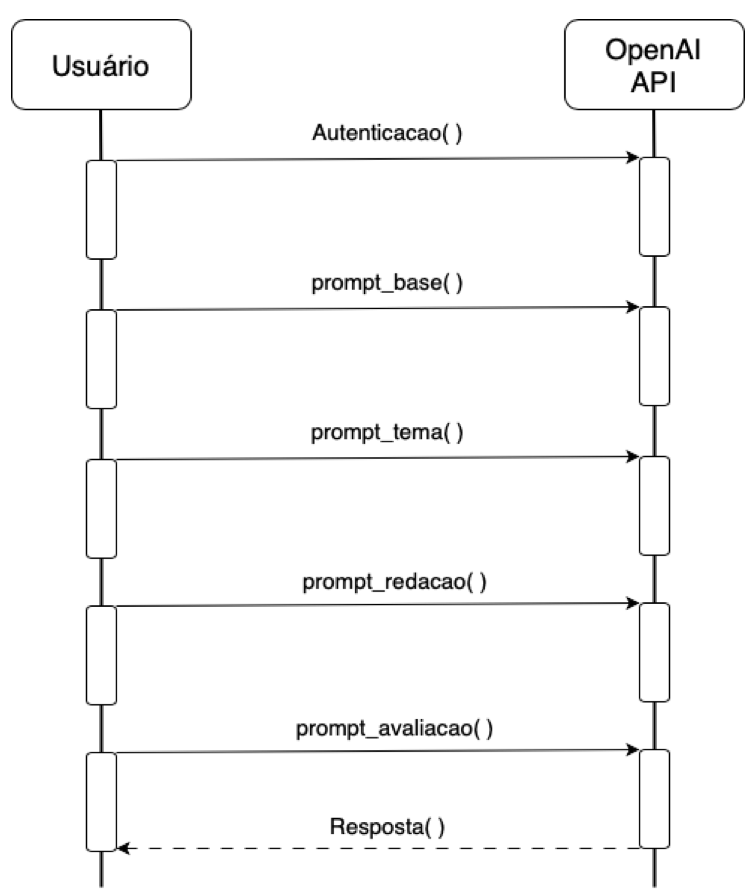
\includegraphics[width=\textwidth]{fig01}
 \caption{Diagrama de Sequência do EnemIA.}
 \label{fig01}
 \source{Elaboração própria.}
\end{minipage}
\end{figure}

O diagrama de sequência \cite{uml} apresentado na \Cref{fig01} ilustra o fluxo de interação entre um usuário, professor ou estudante, e a API (\emph{Application Programming Interface}) da OpenAI, no contexto do EnemIA. Inicialmente, o usuário interage com a API da OpenAI por meio de um processo de autenticação. Esse passo garante a segurança e a personalização dos serviços, verificando a identidade do usuário através de chave e permitindo acesso às funcionalidades do sistema. A autenticação bem-sucedida estabelece uma sessão segura e personalizada para o usuário.
Seguindo a autenticação, a ferramenta envia uma série de prompts à API da OpenAI. 

O primeiro desses prompts, denominado "prompt\_base", estabelece um contexto geral para a redação, o qual inclui informações sobre os critérios de avaliação, as normas gramaticais e estilísticas esperadas, e outras orientações que ajudam a IA a compreender o escopo da tarefa de correção. O próximo passo é o envio do "prompt\_tema", que fornece o tema específico da redação a ser avaliada e contextualiza a IA sobre o tópico em questão. Esta informação avalia a relevância e a profundidade do conteúdo produzido pelo estudante em relação ao tema proposto. Em seguida, o "prompt\_redacao" é enviado, contendo o texto completo da redação produzida pelo estudante. A partir deste ponto, a IA processa o conteúdo da redação, analisando aspectos como coerência, coesão, estrutura argumentativa, clareza e precisão das ideias apresentadas. A análise também abrange a verificação de erros gramaticais e ortográficos, além da adequação ao tema proposto.

Após essa análise, é enviado o "prompt\_avaliacao", que instrui a IA a aplicar os critérios de avaliação específicos do Enem para fornecer um \textit{feedback} detalhado sobre os pontos fortes e fracos da redação, tendo em vista os critérios já citados. Por fim, a ferramenta estrutura a resposta gerada pela IA e a devolve ao usuário com comentários e sugestões de aprimoramento. O \textit{feedback} é detalhado e construtivo, auxiliando o estudante a identificar pontos que necessitam de melhoria e a compreender os critérios de avaliação do Enem com mais clareza. O diagrama de sequência ilustra a eficiência e a precisão da interação entre o usuário e a API da OpenAI, destacando como a inteligência artificial pode apoiar e aprimorar processos de ensino e aprendizagem, especialmente na avaliação de competências complexas, como a produção textual. 

A integração da IA no contexto educacional oferece um potencial significativo para complementar o trabalho dos professores \cite{SacheteSalcedo}, fornecendo uma tecnologia adicional que contribui para a formação de estudantes preparados e conscientes quanto às exigências acadêmicas em relação à redação. Assim, o código foi estruturado para maximizar a eficiência e a precisão na correção, garantindo que todos os critérios sejam considerados de maneira padronizada, o que não apenas reduz a carga de trabalho dos professores, mas também contribui para minimizar a subjetividade inerente ao processo de avaliação humana. Além disso, a aplicação da IA possibilita a geração rápida de \textit{feedback}s detalhados, auxiliando os estudantes a compreenderem melhor seus pontos fortes e áreas que precisam de melhorias.

\section{Metodologia}\label{metodologia}

Diante das projeções previstas no cenário delineado por no Relatório Horizon \cite{educause2023horizon} \cite{vicari2018ia}, e da crescente tendência de integração da IA na educação \cite{loiola2024chatgpt}, decidiu-se desenvolver e avaliar a EnemIA. O objetivo principal desta avaliação foi compreender a eficácia e as limitações do EnemIA como suporte na correção de redações preparatórias para o Enem, bem como investigar seu impacto no processo de ensino-aprendizagem dos estudantes. 

Para tanto, adotou-se uma abordagem qualitativa realizada por meio de uma pesquisa exploratória, adequada ao contexto do uso emergente, porém em rápida evolução, das ferramentas de Inteligência Artificial na Educação. A escolha por esse tipo de investigação justificou-se por sua relevância em áreas inovadoras, em que há necessidade de compreender como essas novas tecnologias podem ser integradas ao ensino e quais são suas possíveis implicações pedagógicas. O objetivo da pesquisa exploratória é aprimorar ideias e revelar novas perspectivas, buscando familiarizar-se com um tema ainda pouco conhecido ou explorado \cite{gil2008projetos}. Seu caráter flexível permite abarcar diferentes aspectos do fenômeno investigado, possibilitando uma abordagem ampla e adaptável à medida que novas percepções surgem durante o processo \cite{gerhardt2009metodos}. Essa flexibilidade favoreceu uma maior familiaridade com o problema, ao mesmo tempo em que revelou lacunas e direcionou futuras investigações.

A abordagem qualitativa recorre a métodos como observação, análise de documentos e entrevistas semiestruturadas para uma exploração aprofundada do fenômeno estudado \cite{ribeiro2024entrevista}, facilitando a coleta de dados sobre o emprego de IA em práticas pedagógicas. A pesquisa qualitativa valoriza os depoimentos dos atores sociais e os significados que expressam, destacando-se pela descrição minuciosa dos fenômenos e seus contextos \cite{vieira2005pesquisa}. Além disso, a análise dos dados seguiu um caminho indutivo, com a pesquisa qualitativa emergindo ao longo do estudo, em vez de ter sido rigidamente pré-definida. 

Dessa maneira, inicialmente, buscou-se embasamento teórico na literatura para o desenvolvimento da EnemIA. Em seguida, comparou-se o sistema com outro semelhante, e, posteriormente, foi integrado à rotina de correção de redações ao longo de um semestre letivo.

Participaram da pesquisa\footnote{Este trabalho integra uma pesquisa aprovada pelo Comitê de Ética em Pesquisa da Universidade Federal do Rio Grande do Sul (UFRGS), conforme Parecer nº 6.720.649.} docentes de Língua Portuguesa e discentes do terceiro ano do ensino médio do curso Técnico em Informática Integrado do Instituto Federal de Educação, Ciência e Tecnologia Farroupilha. A turma, composta por 35 estudantes com idades entre 15 e 17 anos, estava em fase de preparação para o Enem. Todos os participantes assinaram o Termo de Consentimento Livre e Esclarecido (TCLE), e suas identidades foram preservadas, assegurando o anonimato das informações coletadas. A escolha desse grupo foi motivada pela disponibilidade e interesse em participar da pesquisa, além da necessidade de preparar os alunos para o exame nacional. Essa fase também envolveu a configuração inicial do EnemIA, adaptando o prompt base e as instruções de acordo com as necessidades da turma. 

O professor recebeu treinamento sobre o uso da EnemIA e discutiu com os alunos sua implementação no processo de correção das redações. Os estudantes foram instruídos a utilizar a plataforma para redigir seus textos dissertativo-argumentativos sobre temas variados, seguindo o formato exigido pelo Enem. Após, o docente utilizou os \textit{feedback}s gerados pelo sistema para discuti-los com os alunos em sessões individuais e coletivas. A cada mês, os alunos redigiram uma nova redação, totalizando seis redações ao longo do período de estudo. 

Por fim, os alunos registraram suas percepções sobre a utilização da ferramenta. Os dados obtidos foram coletados e analisados qualitativamente, e os resultados serviram de subsídio para o aprimoramento do uso da EnemIA, além de orientar o planejamento de futuras intervenções pedagógicas.

\section{Avaliação}\label{avaliacao}

Esta seção apresenta quatro discussões distintas. A primeira compara a EnemIA com outro recurso online de avaliação de redações do Enem, Redarito. A segunda, refere-se à aplicação da EnemIA em uma turma do terceiro ano do ensino médio, seguida de uma análise qualitativa dos resultados. A terceira apresenta uma avaliação de desempenho que demosntra o antes e o depois da utilização do EnemAI e seu impacto na escrita do estudante. A quarta apresenta as limitações da pesquisa.

\subsection{\textbf{Comparação entre EnemIA e Redarito}}\label{comparacao}

O Redarito é uma plataforma online que analisa e pontua redações de acordo com os requisitos avaliados no Enem. Sua avaliação foi utilizada em termos de comparação com a avaliação realizada pela EnemIA. Na \Cref{fig02}, apresenta-se uma redação nota 1000 do Enem de 2020, cujo tema foi “O estigma associado às doenças mentais na sociedade brasileira”. Escrita pela estudante Julia Vieira, essa redação está publicamente disponível no site BrasilEscola que reúne exemplos de redações nota máxima.

\begin{figure}[htbp]
\centering
\begin{minipage}{\textwidth}
 \fbox{
\includegraphics[width=\textwidth]{fig02}}
 \caption{Exemplo de redação nota 1000 no Enem.}
 \label{fig02}
 \source{\url{https://vestibular.brasilescola.uol.com.br/enem/enem-2020-leia-uma-das-redacoes-nota-1000/349736.html}}
\end{minipage}
\end{figure}

A \Cref{fig03} apresenta a análise realizada, primeiramente pelo Redarito e, em seguida, pela EnemIA (na \Cref{fig04}). A comparação entre essas tecnologias de avaliação de redações revelou abordagens distintas para orientar os estudantes que buscam aprimorar suas produções textuais no contexto do Enem. Embora ambas tenham como objetivo fornecer \textit{feedback}s construtivos, suas estratégias e estilos de comunicação diferem significativamente.

\begin{figure}[htbp]
\centering
\begin{minipage}{\textwidth}
 \fbox{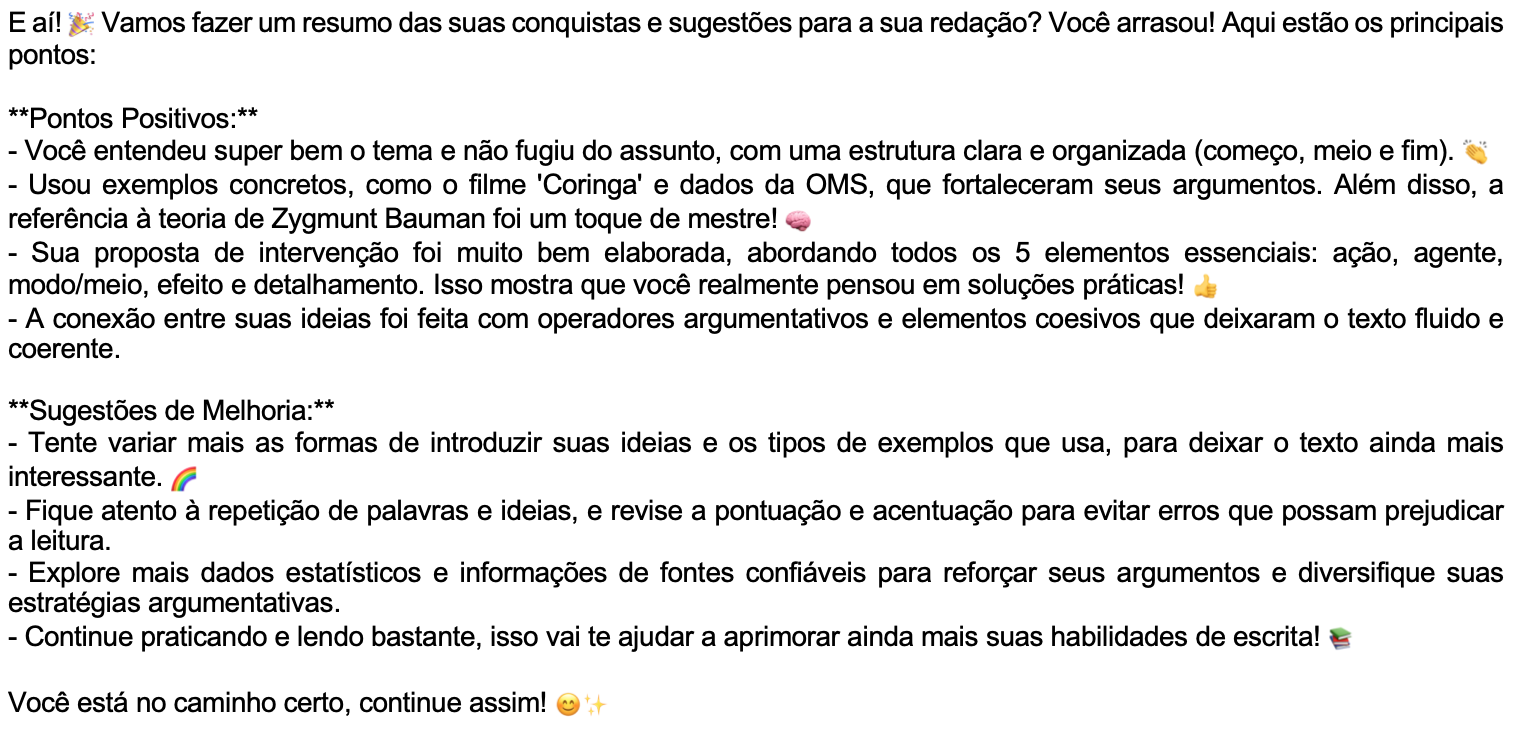
\includegraphics[width=\textwidth]{fig03}}
 \caption{Avaliaçao realizada pelo Redarito.}
 \label{fig03}
\source{Elaboração própria.}
\end{minipage}
\end{figure}

O Redarito adota um tom acolhedor e motivacional, embora superficial em termos de técnica. Seu \textit{feedback} é carregado de emojis, expressões encorajadoras e um toque leve, criando uma experiência que faz o estudante se sentir valorizado desde o início. Expressões como "Você arrasou!" e "Você está no caminho certo, continue assim!" são utilizadas para incentivar a dedicação contínua do aluno, sendo particularmente úteis para aqueles que se sentem inseguros ou desmotivados. O \textit{feedback} do Redarito é dividido entre pontos positivos e sugestões de melhoria, o que facilita a identificação rápida dos pontos fortes e das áreas que necessitam de aperfeiçoamento. 

\begin{figure}[htbp]
\centering
\begin{minipage}{\textwidth}
 \fbox{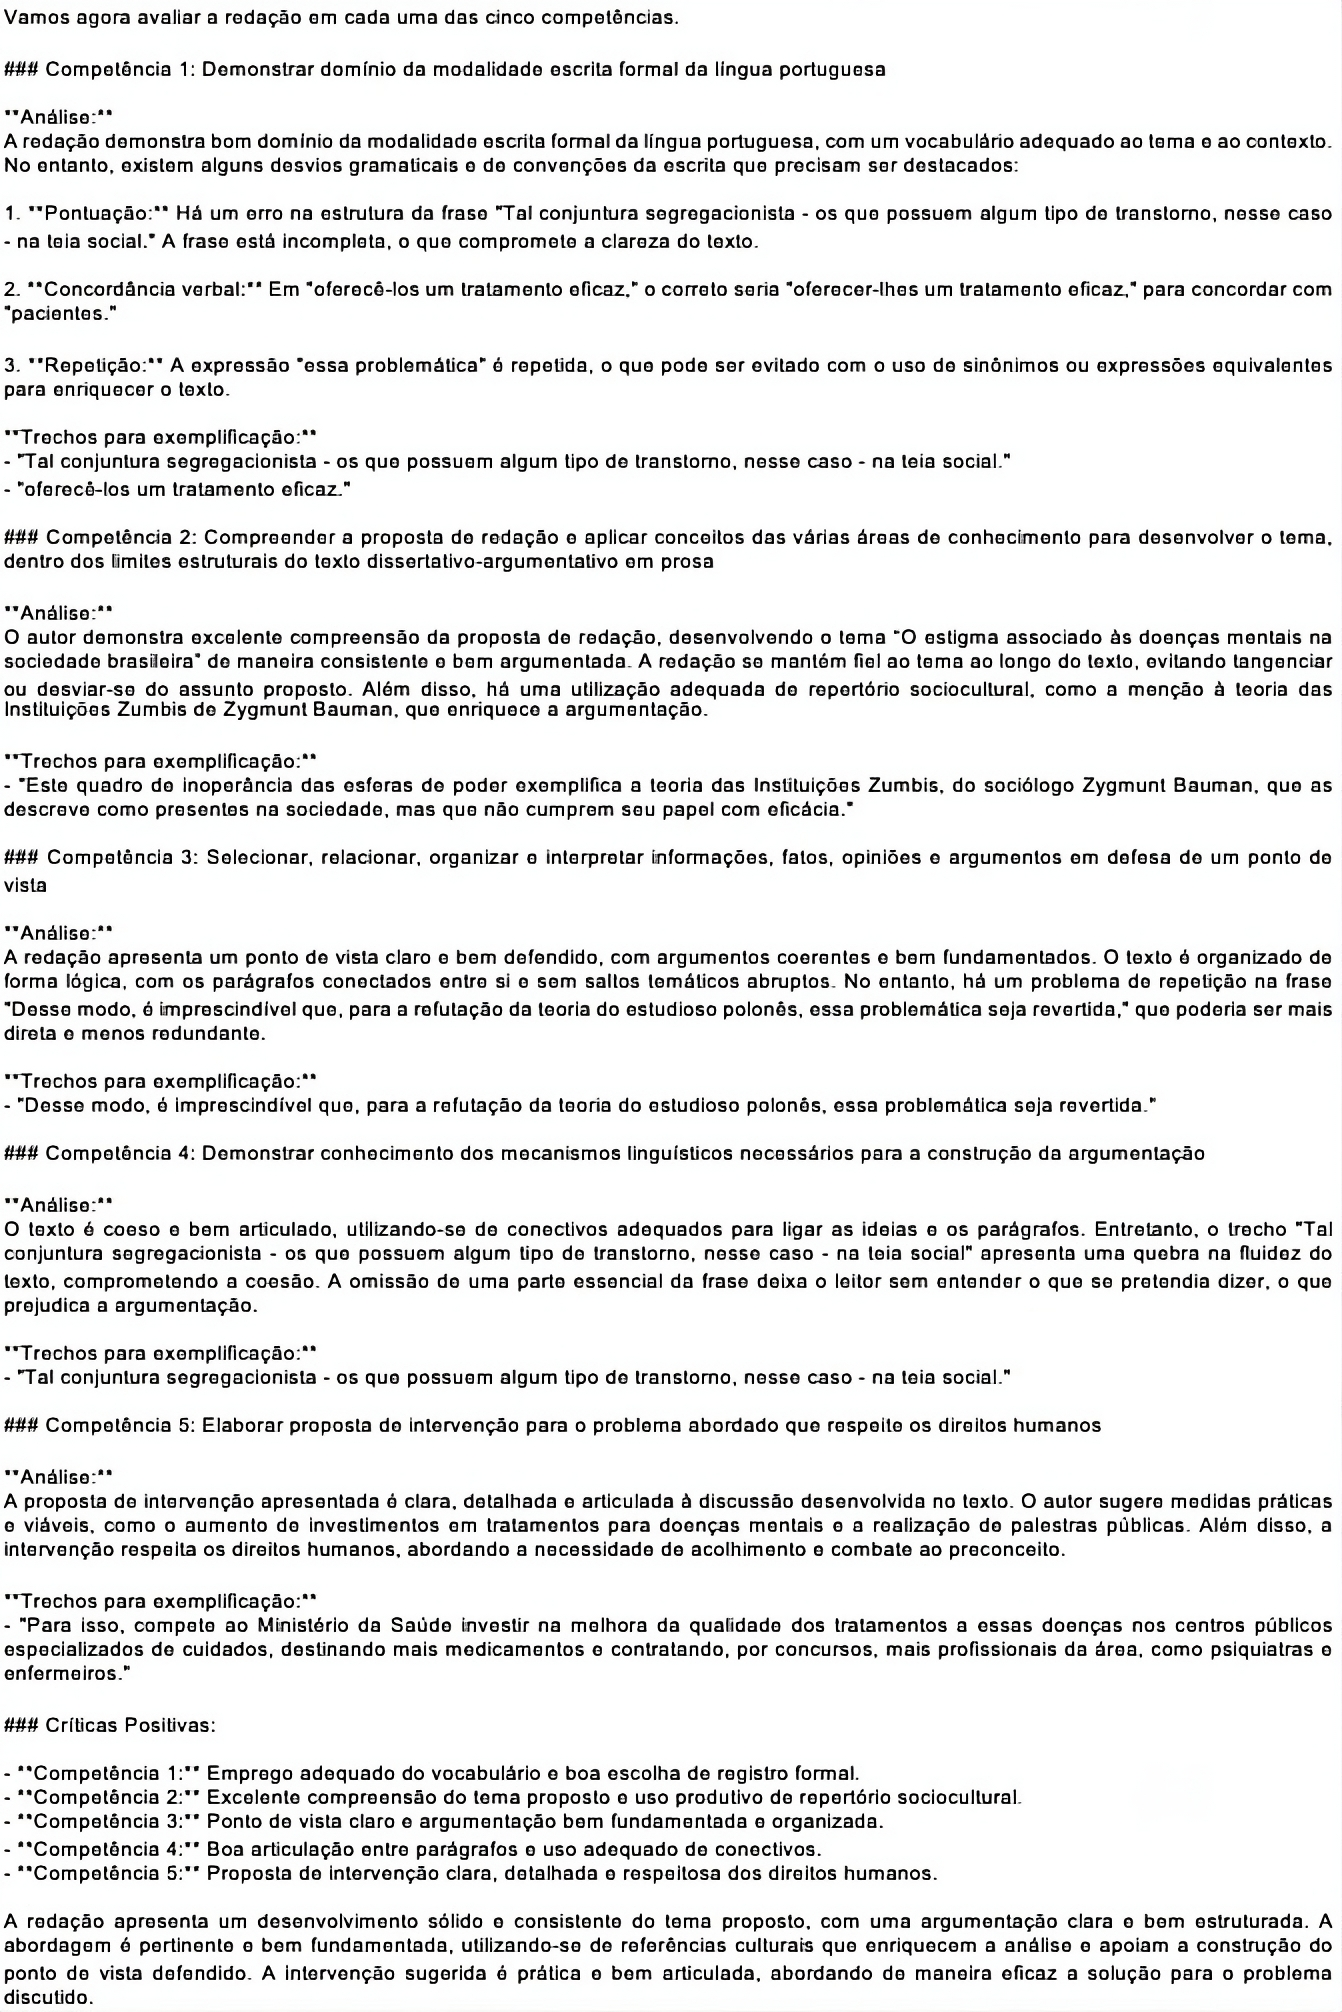
\includegraphics[width=\textwidth]{fig04-2}}
 \caption{Avaliaçao realizada pelo EnemIA.}
 \label{fig04}
 \source{Elaboração própria.}
\end{minipage}
\end{figure}

Entre os aspectos elogiados, destaca-se o reconhecimento do uso de exemplos concretos e teorias, como a menção a Zygmunt Bauman, apontando a relevância dessas referências na argumentação. Além disso, o Redarito também valoriza a proposta de intervenção do estudante, apontando sua adequação aos critérios exigidos pelo Enem e destacando sua qualidade e consistência. No entanto, suas sugestões para o aprimoramento – como variar as formas de introdução de ideias, revisar a pontuação e evitar repetição de palavras – são apresentadas de maneira genérica, sem fornecer exemplos específicos do texto avaliado, o que pode dificultar a compreensão exata dos erros e como corrigi-los. Ou seja, o Redarito pode ser um tanto superficial no \textit{feedback} de sugestões, deixando de oferecer múltiplas alternativas para o aperfeiçoamento de frases e parágrafos, do ponto de vista gramatical, sintático e discursivo-pragmático. A recomendação final para "continuar praticando e lendo bastante" reforça a importância do aprimoramento contínuo, mas carece de maior especificidade no aconselhamento prático.

A EnemIA, como mostrado na \Cref{fig04}, devido ao modo de configuração de sua tecnologia generativa, adota uma abordagem mais técnica e detalhada, com \textit{feedback} estruturado de acordo com as cinco competências do Enem, o que proporciona uma análise minuciosa de cada aspecto da redação. Ao contrário do Redarito, além de ter um tom mais formal e focado nos pontos fortes e fracos da produção, a EnemIA também oferece uma análise segmentada que facilita a identificação das competências que precisam de melhorias. 

A ferramenta se destaca por citar trechos específicos da redação para exemplificar tanto os acertos quanto os erros, o que pode facilitar a compreensão das críticas. A construção de sentidos deve guiar os mecanismos de escrita e como uma correção estanque pode impedir o escritor de desenvolver uma uma reflexão metassemântica mais elaborada \cite{koch2003texto}. Nesse sentido, ao apontar um erro de pontuação, o sistema apresenta o trecho exato em que o erro ocorreu, o que ajuda o estudante a visualizar o problema e corrigir seus equívocos dentro de um contexto de significados. 

Além das questões gramaticais, como concordância verbal e repetição de expressões, a EnemIA faz sugestões claras sobre como melhorar esses aspectos. O uso adequado do repertório sociocultural, como a menção à teoria de Zygmunt Bauman, também é elogiado, reforçando a importância de referências teóricas bem aplicadas. Com uma análise técnica aprofundada e segmentada, a EnemIA é ideal para estudantes que já possuem um certo domínio das competências e querem melhorar suas produções de maneira objetiva.

Ao comparar as duas abordagens, percebe-se que servem a propósitos diferentes dentro do mesmo contexto de avaliação de redação. O Redarito foca em criar uma experiência de aprendizado acolhedora e motivadora, enquanto a EnemIA proporciona uma análise técnica, informativa e direta, segmentada por cada competência, com exemplos específicos do texto do estudante. O Redarito, por sua vez, fornece sugestões mais gerais, sem muitos exemplos específicos.

\subsection{\textbf{Aplicação da EnemIA em Sala de Aula}}

A aplicação de simulados do Enem, aliada aos \textit{feedback}s da EnemIA, iniciou com a introdução de situações-problema, conforme proposto pelo INEP \cite{inep2020edital}. Para tal, foi disponibilizado um texto-base como apoio, e solicitado aos alunos que selecionassem o material mais adequado para auxiliá-los na redação. Cada estudante escolheu um artigo para consultar durante o processo de escrita. Como as redações foram redigidas no computador, estabeleceu-se um limite de 2500 caracteres, incluindo espaços, equivalente a aproximadamente 30 linhas. Essa medida foi adotada para representar a versão manuscrita do exame, reconhecendo variações individuais na escrita, mas considerando essa média como uma aproximação adequada para fins de simulação.

A avaliação qualitativa da utilização da EnemIA baseou-se nos comentários dos estudantes que a utilizaram. A seguir, na \Cref{fig05}, apresentam-se as percepções dos alunos e após discutem-se os principais pontos levantados, destacando as vantagens e limitações da aplicação da inteligência artificial no contexto das redações do Enem.

Um ponto de destaque foi a percepção, por parte de alguns alunos, de que a EnemIA apresentou maior rigor ao destacar pequenos erros que, em geral, poderiam ser desconsiderados por avaliadores humanos. Apesar disso, os estudantes reconheceram o valor da ferramenta como um recurso de aprimoramento, utilizando-a para identificar falhas sutis e aprimorar seu desempenho nas produções textuais. 

\begin{figure}[!htbp]
\centering
\begin{minipage}{\textwidth}
 \fbox{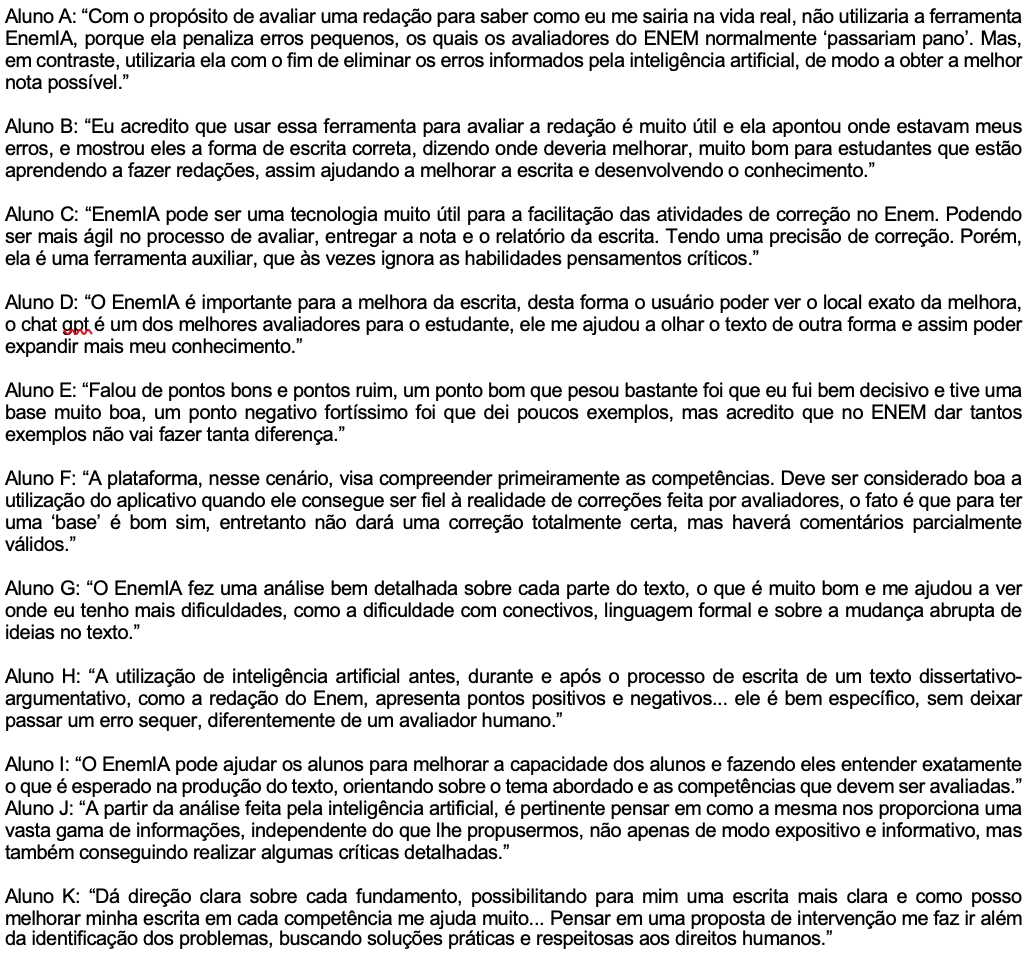
\includegraphics[width=\textwidth]{fig05}}
 \caption{Percepções dos estudantes.}
 \label{fig05}
 \source{Elaboração própria.}
\end{minipage}
\end{figure}

Um dos estudantes elogiou a capacidade da EnemIA de identificar erros específicos, destacando sua utilidade para quem ainda está em processo de aprendizagem. A clareza nas orientações oferecidas pela IA auxilia no desenvolvimento das habilidades de escrita, facilitando o entendimento dos pontos a serem aprimorados. Há uma demanda por produções escritas que se articulem com \textit{feedback}s detalhados, capazes de proporcionar ao aluno uma perspectiva da minúcia de cada aspecto do texto e de como essas características dialogam na formação de um todo significativo \cite{geraldi2011linguagem}.

Outros estudantes também reconheceram o potencial do sistema para otimizar o processo de escrita. Um deles destacou a agilidade nas correções, com análises rápidas e precisas, embora tenha mencionado dificuldades da IA em avaliar o pensamento crítico com a mesma profundidade de um avaliador humano. Além disso, os alunos reconheceram o valor do \textit{feedback} localizado, que proporcionou uma análise mais detalhada e direcionada, contribuindo para a melhoria da estrutura e para coerência das redações. 

Contudo, houve quem mencionasse que a IA, às vezes, focava em aspectos não tão relevantes para o contexto específico do Enem, como o número de exemplos apresentados. Alguns alunos ressaltaram a utilidade da análise detalhada oferecida pela IA, especialmente para identificar áreas específicas de dificuldade, o que reforça a diversidade de percepções entre os usuários.

O papel formativo da EnemIA também foi amplamente reconhecido. Sua precisão foi elogiada por auxiliar na correção de pequenos erros, mesmo que essa rigidez nem sempre corresponda ao critério mais flexível de avaliadores humanos. Outro ponto positivo foi o suporte à organização das ideias, o que permitiu aos alunos refletirem de forma rápida e informada.

Por fim, um dos estudantes destacou que as sugestões do sistema abrangem não apenas aspectos estruturais, mas também argumentativos e éticos, contribuindo de maneira integral para o desenvolvimento da redação. A construção textual deve estar imbricada ao contexto social e inscrever-se nele \cite{dolz2010producao}. Essa leitura social do texto é bastante explorada pelo Enem, mas, geralmente, pouco desenvolvida em sala de aula; logo, esse tipo de \textit{feedback} torna-se mister aos alunos. A pesquisa se destaca em relevância por trazer o discente como protagonista para o processo de análise sobre \textit{feedback} gerado pela ferramenta, ativando processos mentais sobre a própria construção do gênero textual e os mecanismos que garantem clareza e coerência o texto.

De forma geral, a avaliação qualitativa revela que a EnemIA é eficaz no aprimoramento da escrita, especialmente no que tange à organização e à estrutura textual. Embora alguns alunos apontem críticas sobre a rigidez e a falta de flexibilidade em determinados critérios, a maioria reconhece seu valor como uma tecnologia de apoio. As críticas sugerem ajustes que podem aproximar a IA da realidade das avaliações humanas, equilibrando precisão técnica com uma avaliação mais contextualizada.

\subsection{\textbf{Análise Comparativa de Desempenho com EnemIA}}

A seguir, apresentam-se dois parágrafos retirados de textos produzidos pelo mesmo aluno. O primeiro, cujo tema é \textit{O uso do celular em sala de aula}, foi escrito antes da introdução da ferramenta EnemAI. O segundo, que aborda \textit{Tecnologia no ambiente escolar}, foi desenvolvido após seis meses de utilização do recurso.

\begin{itemize}
\item \emph{Aluno - Trecho da Redaçao anterior à EnemIA}. ``O celular é um objeto muito usado hoje em dia. Ele está presente na vida de quase todo mundo. Com ele dá para acessar a internet, redes sociais e também estudar. Muitas escolas estão discutindo se o uso do celular na sala de aula deve ser permitido ou não. Esse assunto é importante porque o celular pode ajudar no aprendizado, mas também pode atrapalhar.''

\item \emph{Aluno - Trecho da Redaçao posterior à EnemIA}. ``Hoje em dia, com o avanço da tecnologia, é normal ver o uso de ferramentas digitais nas aulas. Sites educativos, vídeos e até inteligência artificial estão mudando a forma como a gente aprende. Mas, mesmo sendo muito úteis, essas tecnologias precisam ser usadas com cuidado e planejamento, para que todos os alunos tenham as mesmas chances e a educação seja realmente boa para todo mundo.''
\end{itemize}

A comparação entre os dois textos evidencia uma evolução na escrita do aluno após a utilização da EnemAI. Observa-se maior elaboração das ideias, com argumentos mais consistentes e postura crítica mais evidente. Além disso, há melhorias na coesão textual, no uso de conectivos e na ampliação do vocabulário, que se apresenta mais técnico e apropriado ao tema. Esses avanços apontam que a ferramenta contribuiu para o aprimoramento da capacidade argumentativa, da organização do texto e da qualidade da linguagem empregada.

\subsection{\textbf{Limitações da Pesquisa}}

Existem diretrizes iniciais para a realização da prova de redação do Enem que a EnemIA, em sua versão atual, não consegue identificar. A EnemIA é um recurso de apoio para utilização em sala de aula, destinada a auxiliar os processos de ensino e aprendizagem de redações escritas pelos estudantes em um editor de textos. Entretanto, não consegue contabilizar a quantidade mínima de linhas, pois isso depende do tamanho da letra do aluno e do espaço na folha de prova, variáveis que não são reproduzíveis com precisão no ambiente computacional. Além disso, questões como rasuras, assinaturas, nomes ou desenhos não são considerados nessa implementação.

Outro ponto é que a EnemIA não atribui nota à redação. Essa escolha foi tomada pelos desenvolvedores diante do elevado risco de erro na pontuação. Ao analisar as Tabelas de desempenho por competência, pode-se observar que a diferença entre os \textit{steps} dentro da mesma competência é de 40 pontos (200, 160, 120, 80, 40 e 0). Assim, um equívoco na avaliação de apenas um nível em cada competência pode gerar uma diferença de até 200 pontos na nota final. Por exemplo, uma redação que deveria ser pontuada com 1000 pontos, recebendo 200 em cada uma das cinco competências, poderia ser pontuada com 160 em cada competência, resultando em uma nota final de 800. Portanto, a diferença de 40 pontos entre cada step tem impacto significativo na pontuação final.

Ademais, a IA generativa apresenta limitações na avaliação textual. Seu treinamento em grandes quantidades de dados, abrangendo diversos estilos de escrita e normas gramaticais, a faz optar por um step mais baixo de avaliação, dada sua tendência a identificar incoerências e inconsistências textuais, como mudanças bruscas de tom ou falta de clareza nas ideias. Esse processo lhe confere uma compreensão profunda do que é considerado um texto bem-escrito em diferentes contextos. A IA também é sensível a erros gramaticais e ortográficos, aplicando regras rigorosas para identificar e corrigir essas falhas, o que pode tornar sua avaliação mais crítica. Ela verifica a precisão e relevância das informações sem influências emocionais ou preconceitos, o que assegura uma análise objetiva, baseada em critérios predefinidos. No entanto, sua rigidez na identificação de padrões, como repetições desnecessárias e o uso inadequado de figuras de linguagem, pode resultar em uma avaliação mais rigorosa que a de leitores humanos. 

Por fim, a aplicação da inteligência artificial na correção de redações ainda impõe desafios importantes. Embora contribua para reduzir a sobrecarga dos docentes, seu uso deve ser cauteloso, a fim de garantir que complemente e fortaleça a avaliação pedagógica, sem substituí-la. Para isso, é essencial que os professores estejam devidamente capacitados, sabendo utilizar a tecnologia de forma adequada ao contexto de ensino e interpretar seus resultados de maneira crítica e contextualizada.

\section{Considerações Finais}\label{consideracoes}

A avaliação de redações no ambiente escolar representa um desafio recorrente, sobretudo em turmas do ensino médio marcadas pela heterogeneidade de níveis de proficiência, estilos e ritmos de aprendizagem. Diante desse panorama, esta pesquisa propôs-se a investigar como o uso de ferramentas baseadas em inteligência artificial pode contribuir para o ensino e a avaliação da escrita nesse contexto.

Os resultados indicaram que a EnemIA é uma alternativa eficaz para auxiliar na correção das redações. Ao fornecer devolutivas alinhadas aos critérios do Enem, a ferramenta auxiliou os estudantes na identificação de aspectos específicos a serem aprimorados, contribuindo para o desenvolvimento de suas competências textuais. 

Os participantes relataram que o \textit{feedback} foi claro, objetivo e instrumental na reescrita dos textos.
Do ponto de vista docente, a utilização da ferramenta contribuiu para a otimização do tempo destinado à correção, permitindo-lhes concentrar-se em estratégias pedagógicas personalizadas. Dessa forma, a EnemIA revelou-se uma aliada tanto na avaliação quanto no ensino da escrita, especialmente quando adaptada às necessidades da prática escolar. 

A incorporação dessa tecnologia representa um avanço ao articular a agilidade da IA generativa com a mediação docente. Ao automatizar tarefas operacionais, como a análise inicial das produções, a ferramenta favorece um ambiente de aprendizagem mais interativo e centrado no processo formativo.

Num cenário em que as práticas discursivas são cada vez mais mediadas por tecnologias digitais \cite{gomes2018generos}, a aplicação da inteligência artificial na educação surge como uma oportunidade para enriquecer os processos avaliativos e potencializar o ensino de redação. Sua capacidade de ampliar a personalização e fortalecer a avaliação contínua aponta para caminhos promissores na formação dos estudantes, especialmente frente aos desafios impostos pelo Enem.

\printbibliography\label{sec-bib}
% if the text is not in Portuguese, it might be necessary to use the code below instead to print the correct ABNT abbreviations [s.n.], [s.l.]
%\begin{portuguese}
%\printbibliography[title={Bibliography}]
%\end{portuguese}


%full list: conceptualization,datacuration,formalanalysis,funding,investigation,methodology,projadm,resources,software,supervision,validation,visualization,writing,review
\begin{contributors}[sec-contributors]
\authorcontribution{Andréia dos Santos Sachete}[conceptualization,investigation,methodology,projadm,writing,review]
\authorcontribution{Alba Valéria de Sant'Anna de Freitas Loiola}[investigation,methodology,review]
\authorcontribution{Ânderson Martins Pereira}[datacuration,investigation,writing]
\authorcontribution{Fábio Diniz Rossi}[formalanalysis,software,validation,writing,review]
\authorcontribution{Raquel Salcedo Gomes}[supervision,writing,review]
\end{contributors}


\end{document}

